\documentclass[conference,10pt]{IEEEtran}
\usepackage[utf8]{inputenc}
\usepackage[T1]{fontenc}
\usepackage[spanish,es-noshorthands]{babel}
\usepackage{amsmath,amssymb,amsthm}
\usepackage{algorithm}
\usepackage[noend]{algpseudocode}
\usepackage{graphicx}
\usepackage{booktabs}
\usepackage{url}
\usepackage[hidelinks]{hyperref}
\usepackage{cite}

\newtheorem{proposition}{Proposición}
\newtheorem{lemma}{Lema}
\floatname{algorithm}{Algoritmo}
\renewcommand{\algorithmicrequire}{\textbf{Entrada:}}
\renewcommand{\algorithmicensure}{\textbf{Salida:}}
\newcommand{\tok}{\operatorname{tok}}
\newcommand{\Sterm}{S}

\begin{document}

\title{Árbol de Steiner consciente de tokens\\para consultas de movilidad urbana en LLMs}

\author{\IEEEauthorblockN{David Rangel Monsiváis, Damián Alejandro Gómez Mena, Gael Alexandor Zaragoza Torres}
\IEEEauthorblockA{Equipo 7 \textperiodcentered{} TC2038 Análisis y Diseño de Algoritmos Avanzados \textperiodcentered{} Tecnológico de Monterrey\\
Midterm 1 \textperiodcentered{} 21 de octubre de 2026}}

\maketitle

\begin{abstract}
Un LLM que responde consultas de movilidad no puede recibir el grafo vial de una zona metropolitana: el grafo de solo el centro de Monterrey serializado ocupa 254{,}893 tokens. Proponemos una herramienta MCP que, dada la consulta ya interpretada por el LLM (origen, destino y puntos de interés), devuelve un subgrafo podado mediante un Árbol de Steiner con pesos conscientes de tokens, una ruta ordenada exacta sobre ese subgrafo (Held--Karp) con reparación dirigida, y una serialización con contracción de cadenas. Presentamos la formalización, la correctitud, la complejidad y una cota de aproximación para la relajación simétrica, junto con un experimento preliminar sobre 150 consultas fijas en tres zonas de OpenStreetMap: el método reduce los tokens del prompt entre 9$\times$ y 119$\times$ frente al grafo completo (la razón crece con el grafo), con 100\% de rutas válidas, costo medio a 2.5--4.9\% del óptimo y salida determinista bit a bit. También reportamos un resultado negativo: el peso por arista consciente de tokens no reduce el texto serializado, porque ignora la contracción; proponemos la corrección.
\end{abstract}

\section{Panorama del proyecto}
\textbf{Problema real.} Las consultas de navegación en lenguaje natural traen varios puntos de interés (POI) y preferencias (\guillemotleft{}del Tec a la Macroplaza pasando por una farmacia y un banco, sin peajes\guillemotright{}). Enviar el mapa completo al LLM excede la ventana de contexto, encarece cada consulta de forma lineal en tokens y degrada la calidad: los modelos usan mal la información enterrada en contextos largos~\cite{liu2024lost} y pueden inventar calles.
\textbf{Arquitectura.} El LLM actúa como orquestador vía MCP~\cite{mcp2024}: (1)~extrae entidades y restricciones; (2)~llama a la herramienta \texttt{plan\_route}; (3)~nuestro algoritmo filtra, poda y ordena; (4)~devuelve un texto compacto de a lo más $B$ tokens; (5)~el LLM verbaliza las instrucciones. El \emph{LLM decide} qué restricciones semánticas aplicar y cómo redactar; el \emph{algoritmo decide} qué calles entran al contexto y en qué orden se visitan los POI.
\textbf{Requisitos.} Recurso optimizado: tokens de entrada (costo y latencia de \emph{prefill}). Calidad: ruta 100\% válida sobre el grafo, cobertura total de POI, costo a no más de 10\% del óptimo ($\rho\le 1.1$). Datos: OpenStreetMap vía OSMnx~\cite{boeing2017}, usado solo para obtener el grafo; Dijkstra, Steiner, Held--Karp, Kruskal y la serialización son implementación propia.

\section*{Parte I --- Análisis algorítmico}

\section{Q1. Definición, motivación y supuestos}
\textbf{Entradas.} Un grafo dirigido $G=(V,E)$, $n=|V|$, $m=|E|$, fuertemente conexo, con tiempo de recorrido $t:E\to\mathbb{R}_{>0}$ y nombre de calle por arista. Una consulta $q=(s,d,P,C)$ con origen $s$, destino $d$, POI $P=\{p_1,\dots,p_k\}\subseteq V$ y restricciones $C$ (aristas prohibidas). Terminales $\Sterm=\{s,d\}\cup P$, $\ell=|\Sterm|$. Un presupuesto de contexto $B$ y un serializador $\sigma$ con conteo de tokens $\tok(\cdot)$.

\textbf{Salidas.} Un subgrafo $H\subseteq G_C$ ($G$ sin las aristas de $C$) y un recorrido $R=(s,\dots,d)$ en $H$ que visita todo $P$, entregados como el texto $\sigma(H,R)$.

\textbf{Objetivos (en conflicto).}
\begin{align}
f_1 &= \tok(\sigma(H,R)) && \text{(dominio computacional)}\\
f_2 &= c(R)=\textstyle\sum_{e\in R} t(e) && \text{(dominio físico)}
\end{align}
sujeto a: $R$ válido en $G$ (cada par consecutivo es arista), $P\subseteq R$, $H$ conecta $\Sterm$ y $f_1\le B$. Se escalariza con $w_\lambda(e)=t(e)+\lambda\,\tau(e)$, donde $\tau(e)$ es el costo en tokens de serializar $e$; la hipótesis es que barrer $\lambda$ traza el frente de Pareto entre $f_1$ y $f_2$ (refutada para el $\tau$ actual, ver M2).

\textbf{Modelo computacional.} RAM con aritmética real; el LLM es una caja negra cuyo costo es $p_\text{in}f_1+p_\text{out}\,\text{tokens}_\text{out}$ y cuya latencia de \emph{prefill} crece al menos linealmente con $f_1$.

\textbf{Por qué Steiner.} Conectar exactamente $\Sterm$ con la red más barata es el problema de Árbol de Steiner en grafos, NP-difícil~\cite{karp1972}. Un camino Hamiltoniano sobre $V$ sería incorrecto (obliga a visitar todo); concatenar caminos mínimos fija un orden arbitrario y no comparte calles. El Árbol de Steiner es la estructura mínima que contiene un camino entre \emph{cualquier} par de terminales, por lo que sirve para cualquier orden de visita sin otra llamada a la herramienta.

\textbf{Supuestos.} (A1)~El LLM resuelve cada POI a un nodo (\emph{entity linking}); los POI por categoría quedan como trabajo futuro (Q5). (A2)~Tiempos estáticos derivados de límites de velocidad de OSM. (A3)~El árbol se calcula sobre la simetrización $t^{\leftrightarrow}(\{u,v\})=\min(t(u,v),t(v,u))$, porque el Steiner dirigido solo admite aproximaciones $O(\ell^\varepsilon)$~\cite{charikar1999}; la dirección se recupera en la etapa de ruta. (A4)~$k$ pequeño ($k\le 12$), realista para consultas humanas. (A5)~\texttt{o200k\_base}~\cite{tiktoken} como tokenizador de referencia.

\section{Q2. Algoritmo central y correctitud}
\begin{algorithm}[t]
\caption{\textsc{TokenSteinerRoute}$(G,s,d,P,B,\Lambda)$}\label{alg:main}
\begin{algorithmic}[1]
\Require grafo $G$, terminales, presupuesto $B$, rejilla creciente $\Lambda$
\Ensure texto $\sigma$ con $\tok(\sigma)\le B$ (o el mejor esfuerzo)
\State $\tau \gets$ costo en tokens por arista \Comment{precómputo, $O(m)$}
\For{$\lambda\in\Lambda$ en orden creciente}
  \State $U_\lambda \gets$ simetrización de $G$ con $w_\lambda$
  \State $T \gets \textsc{Mehlhorn}(U_\lambda,\Sterm)$ \Comment{Voronoi + MST + poda}
  \State $H \gets \{(u,v)\in E : \{u,v\}\in T\}$ \Comment{reorientar}
  \State $(R,H) \gets \textsc{RutaOrdenada}(G,H,s,d,P)$
  \State $\sigma \gets \textsc{Serializar}(H,R)$ \Comment{contracción de cadenas}
  \If{$\tok(\sigma)\le B$} \Return $\sigma$ \EndIf
\EndFor
\State \Return $\sigma$ marcado como \emph{fuera de presupuesto}
\Statex
\Procedure{RutaOrdenada}{$G,H,s,d,P$}
  \For{$a\in\Sterm$; $b\in\Sterm\setminus\{a\}$}
    \State $D[a,b],\pi_{ab}\gets$ Dijkstra dirigido en $H$ desde $a$
    \If{$b$ inalcanzable en $H$} \Comment{calle de un sentido}
      \State $\pi_{ab}\gets$ Dijkstra en $G$; $H\gets H\cup\pi_{ab}$ \Comment{reparación}
    \EndIf
  \EndFor
  \State orden $\gets$ \textsc{HeldKarp}$(D,s,d,P)$
  \State \Return concatenación de $\pi$ según el orden, $H$
\EndProcedure
\end{algorithmic}
\end{algorithm}

\textbf{Componentes.} \textsc{Mehlhorn}~\cite{mehlhorn1988}: un Dijkstra multi-fuente~\cite{dijkstra1959} desde $\Sterm$ particiona $V$ en celdas de Voronoi; cada arista frontera $(u,v)$ propone la arista $(r_u,r_v)$ de costo $\delta(u)+w(u,v)+\delta(v)$; el MST (Kruskal) de ese grafo se expande a caminos, se recalcula el MST del subgrafo resultante y se podan hojas no terminales. \textsc{HeldKarp}~\cite{heldkarp1962}: $\mathrm{DP}[X,j]=\min_{i\in X\setminus\{j\}}\mathrm{DP}[X\setminus\{j\},i]+D[i,j]$ sobre subconjuntos $X\subseteq P$.

\textbf{Contribución algorítmica.} No aplicamos un Steiner ``de catálogo'': (i)~el \emph{peso consciente de tokens} $w_\lambda$ y el lazo sobre $\lambda$ que ajusta la poda al presupuesto $B$ (implementado; su proxy actual falla, ver M2 y Q5); (ii)~la \emph{contracción de cadenas}: un nodo no terminal de grado 2 cuyas dos aristas son de la misma calle y el mismo sentido se funde, y los ids OSM se renombran a ids locales; (iii)~la \emph{ruta ordenada con reparación dirigida}, necesaria porque un árbol no es una ruta: no fija el orden de visita y, al reorientar, puede perder caminos dirigidos.

\textbf{Invariantes.} (I1)~Dijkstra: al extraer $u$ del heap, $\delta(u)$ es la distancia mínima (pesos no negativos) y $r_u$ es el terminal más cercano. (I2)~Kruskal: el conjunto elegido es siempre un bosque contenido en algún MST. (I3)~Durante \textsc{RutaOrdenada}, $H\subseteq E$ y toda distancia en $D$ corresponde a un camino dirigido real. (I4)~La poda solo elimina hojas $\notin\Sterm$, por lo que $T$ sigue conectando $\Sterm$.

\begin{proposition}[Validez]
Si $G$ es fuertemente conexo, \textsc{TokenSteinerRoute} termina y devuelve una ruta $R$ válida en $G$ que inicia en $s$, termina en $d$ y visita todo $P$.
\end{proposition}
\begin{proof}[Esbozo]
Por (I3) cada $\pi_{ab}$ es un camino en $G$; si no existe en $H$ la reparación lo toma de $G$, que existe por conexidad fuerte. Hay a lo sumo $\ell(\ell-1)$ reparaciones. La concatenación según el orden de Held--Karp empieza en $s$, termina en $d$ y pasa por cada $p_i$.
\end{proof}

\begin{proposition}[Contracción sin pérdida]
Las distancias dirigidas entre nodos no contraídos y la conectividad de $H$ son idénticas antes y después de contraer.
\end{proposition}
\begin{proof}[Esbozo]
Un nodo contraído $x$ tiene exactamente dos vecinos y, si la calle es de un sentido, una arista entra y otra sale; todo camino que toca $x$ lo atraviesa, así que reemplazar la cadena por una arista con tiempo sumado preserva caminos y costos (homeomorfismo de grafos). Los terminales nunca se contraen.
\end{proof}

\textbf{Optimalidad.} Held--Karp es exacto sobre la métrica $D_H$; si $H=G$, la ruta es óptima ($\rho=1$), y así calculamos la referencia.

\section{Q3. Complejidad, garantías y límites}
\textbf{Tiempo.} Dijkstra con heap binario: $O((n+m)\log n)$. \textsc{Mehlhorn}: un Dijkstra multi-fuente, un barrido de aristas y dos Kruskal: $O(m\log n)$ (con heap de Fibonacci~\cite{fredman1987}, $O(m+n\log n)$). \textsc{RutaOrdenada}: $\ell$ Dijkstra sobre $H$, $O(\ell\,|H|\log|H|)$, más $r\le\ell(\ell-1)$ reparaciones de $O(m\log n)$. Held--Karp: $O(2^k k^2)$ tiempo y $O(2^k k)$ espacio. Serialización: $O(|H|)$ más el tokenizador, lineal en la longitud del texto. Total:
\[
O\!\left(|\Lambda|\,\big[(1+r)\,m\log n+\ell|H|\log|H| + 2^k k^2\big]\right),
\]
dominado por $m\log n$ para $k\le 12$. \textbf{Espacio:} $O(n+m+2^k k)$.

\textbf{Garantías.} Para el árbol, $w_\lambda(T)\le 2(1-1/\ell)\,\mathrm{OPT}^{\text{St}}_\lambda$~\cite{kmb1981,mehlhorn1988}; el mejor factor conocido es $\ln 4+\varepsilon\approx1.39$~\cite{byrka2013}, a un costo práctico mucho mayor. Para la ruta en la relajación simétrica sin reparaciones ($\lambda=0$):
\begin{lemma}
$c(R)\le 4(1-1/\ell)\,c(R^*)$, con $R^*$ la ruta óptima.
\end{lemma}
\begin{proof}[Esbozo]
Las aristas de $R^*$ forman un subgrafo conexo que contiene $\Sterm$, luego $c(R^*)\ge\mathrm{OPT}^{\text{St}}$. Un recorrido en profundidad de $T$ desde $s$ que termina en $d$ visita todos los terminales con costo $\le 2w(T)$; Held--Karp sobre $D_T$ no es peor. Por tanto $c(R)\le 2w(T)\le 4(1-1/\ell)\mathrm{OPT}^{\text{St}}\le 4(1-1/\ell)c(R^*)$.
\end{proof}
La cota es de peor caso; empíricamente $\rho$ es mucho menor (Sec.~\ref{sec:m1}). Con calles de un sentido la cota no se sostiene (las reparaciones rompen la estructura de árbol), y la exactitud de la ruta depende de $H$, no de $G$.

\textbf{Límites.} Held--Karp es exponencial en $k$: para $k>15$ se requiere una heurística (vecino más cercano + 2-opt). La monotonía de $f_1$ en $\lambda$ no está garantizada (Mehlhorn es aproximado y $\tau$ es un proxy); el lazo usa $\lambda$ creciente y se detiene en el primero que cumple $B$. El término $r\,m\log n$ no es teórico: observamos $r\approx14$--$19$ reparaciones por consulta, y domina el tiempo en grafos grandes. \textbf{Paralelismo (HPC):} los $\ell$ Dijkstra de \textsc{RutaOrdenada} y los valores de $\Lambda$ son independientes (paralelismo trivial, sin comunicación salvo reunir $D$, $O(\ell^2)$ números); no es el foco del proyecto.

\section{Q4. Robustez, escalabilidad y calidad}
\textbf{Comparación.} \emph{B0}: grafo completo (sin optimizar). \emph{B1}: Dijkstra concatenado en el orden en que el usuario nombró los POI. \emph{B2}: recuperación local tipo RAG~\cite{lewis2020rag}: calles a $\le 250$\,m de la poligonal entre terminales. \emph{M}: propuesto. \emph{REF}: solo la ruta óptima (Held--Karp sobre $G$), cota inferior de tokens y respuesta de referencia. Todos usan el mismo serializador, de modo que las diferencias se deben solo a la selección de calles.

\textbf{Carga creciente.} Tres ejes: tamaño del grafo ($n$ de $\sim\!600$ a $\sim\!12{,}000$ nodos), número de POI ($k\in\{1,2,3,4,6\}$) y presupuesto $B$ (barrido de $\lambda$). B0 crece como $\Theta(m)$ tokens y deja de caber en una ventana de 128k tokens con pocas decenas de miles de aristas; M crece con el tamaño del árbol, $O(\ell\cdot\text{diámetro})$, casi independiente de $n$. B2 depende de la geometría y no garantiza conectividad: su ruta puede no existir.

\textbf{Métricas de calidad (condiciones idénticas).} \emph{Correctitud}: validez de la ruta (cada par consecutivo es arista de $G$) y $\rho=c(R)/c(R^*)$. \emph{Completitud}: fracción de POI cubiertos y de restricciones $C$ respetadas. A nivel LLM: la respuesta se convierte a una secuencia de calles y se compara con $R$ (coincidencia exacta y distancia de edición normalizada); se cuentan calles inexistentes en $H$ (alucinaciones). \emph{Consistencia}: $N=10$ repeticiones por consulta con el mismo modelo fijado por versión, misma plantilla, \texttt{top\_p}$=1$, semilla fija y $T\in\{0,0.7\}$; se reporta la fracción de pares de respuestas con la misma secuencia de calles y la invarianza ante 3 paráfrasis de la consulta.

\section{Q5. Limitaciones y siguientes pasos}
\textbf{L1. El proxy de tokens está mal alineado} (evidencia en M2): $\tau(e)$ por arista ignora la contracción. \emph{Mejora:} cobrar tokens por \emph{cambio de calle}, con peso en los nodos donde cambia el nombre; esto da un Steiner con pesos en nodos, aproximable a $O(\ln\ell)$~\cite{klein1995}, o un Steiner sobre el grafo de líneas. \emph{Evaluación:} correlación de Spearman entre $\lambda$ y tokens (esperada negativa) y frente de Pareto no dominado en las mismas consultas.
\textbf{L2. El árbol restringe la ruta}: $\rho_{95}=1.11$--$1.24$ cuando el árbol no contiene el camino óptimo, y un árbol no ofrece rutas alternativas. \emph{Mejora:} $H'=T\cup R^*$ garantiza $\rho=1$ por construcción, pues Held--Karp sobre $G$ ya se calcula; costo esperado: a lo más los tokens de REF adicionales. \emph{Evaluación:} $\Delta f_1$ contra $\Delta\rho$ en las 150 consultas.
\textbf{L3. POI por categoría} (\guillemotleft{}una farmacia\guillemotright{}) convierten el problema en \emph{Group Steiner Tree}, con aproximación polilogarítmica~\cite{garg2000}. \emph{Mejora:} preselección de $g$ candidatos por categoría por vecinos más cercanos y Held--Karp generalizado sobre grupos, $O(2^k g^2k^2)$. \emph{Evaluación:} $\rho$ contra la enumeración exhaustiva en instancias pequeñas.

\section*{Parte II --- Reporte de avance}

\section{M1 --- Algoritmo central (implementado)}\label{sec:m1}
\textbf{Implementado} (Python 3.13, $\sim$400 líneas propias): Dijkstra multi-fuente, DSU/Kruskal, Steiner de Mehlhorn, poda de hojas, Held--Karp, ruta ordenada con reparación, peso $w_\lambda$, lazo de presupuesto, serializador (lista y JSON) con contracción, baselines B0--B2 y REF. Validado con 6 pruebas: Dijkstra coincide con NetworkX en distancias; el árbol es árbol, contiene $\Sterm$ y sus hojas son terminales; Held--Karp coincide con fuerza bruta; toda ruta de M es válida y $\rho\ge1$.

\begin{table}[t]
\caption{Experimento preliminar: medianas sobre 50 consultas por zona ($k=1,2,3,4,6$; 10 c/u). Tokens en formato lista (\texttt{o200k\_base}); tiempo y memoria pico del algoritmo, sin LLM; $\bar\rho$ y $\rho_{\text{máx}}$ sobre rutas válidas.}\label{tab:prelim}
\centering\footnotesize\setlength{\tabcolsep}{3pt}
\begin{tabular}{llrrrrrr}
\toprule
Zona ($n$) & Mét. & Tokens & ms & KB & Válidas & $\bar\rho$ & $\rho_{\text{máx}}$\\
\midrule
tec {\scriptsize(591)} & B0 & 10,247 & 5.9 & 361 & --- & --- & ---\\
 & B1 & 508 & 1.6 & 122 & 50/50 & 1.250 & 1.942\\
 & B2 & 4,055 & 6.9 & 191 & 18/50 & 1.008 & 1.033\\
 & M & 1,094 & 10.3 & 372 & 50/50 & 1.049 & 1.499\\
 & REF & 476 & 3.5 & 160 & 50/50 & 1.000 & 1.000\\
\midrule
corredor {\scriptsize(2,204)} & B0 & 45,837 & 26.1 & 1,807 & --- & --- & ---\\
 & B1 & 622 & 6.3 & 489 & 50/50 & 1.270 & 1.992\\
 & B2 & 9,572 & 15.1 & 348 & 7/50 & 1.118 & 1.236\\
 & M & 1,352 & 30.5 & 1,659 & 50/50 & 1.025 & 1.234\\
 & REF & 537 & 13.2 & 631 & 50/50 & 1.000 & 1.000\\
\midrule
centro {\scriptsize(11,509)} & B0 & 254,893 & 166.0 & 9,735 & --- & --- & ---\\
 & B1 & 854 & 37.4 & 2,493 & 50/50 & 1.219 & 1.828\\
 & B2 & 21,920 & 74.4 & 975 & 0/50 & --- & ---\\
 & M & 2,136 & 290.0 & 8,185 & 50/50 & 1.047 & 1.481\\
 & REF & 702 & 119.3 & 4,858 & 50/50 & 1.000 & 1.000\\
\bottomrule
\end{tabular}
\end{table}

\textbf{Resultados preliminares (Tabla~\ref{tab:prelim}, Fig.~\ref{fig:tokens}).} (1)~\emph{Eficiencia}: M usa 9.4$\times$, 33.9$\times$ y 119$\times$ menos tokens que B0; B0 en el centro (254{,}893) ya excede ventanas de 128k y 200k tokens, mientras M crece de 1{,}094 a 2{,}136 tokens con un grafo 19 veces mayor. M cuesta 2.3--3$\times$ los tokens de REF (solo la ruta) a cambio de entregar la red que conecta todos los terminales. (2)~\emph{Calidad}: 100\% de rutas válidas en M; $\bar\rho$ de 1.025--1.049 y $\rho=1$ exacto en 58--64\% de las consultas, pero el percentil 95 es 1.11--1.24: la meta $\rho\le1.1$ \emph{aún no se cumple} en la cola (L2 en Q5). B1 empeora con $k$ ($\bar\rho=1$ con $k=1$, 1.40--1.57 con $k=6$) porque no optimiza el orden; B2 no conecta los terminales en 64\%, 86\% y 100\% de las consultas. (3)~\emph{Reparación}: las 150 consultas de M necesitaron reparaciones dirigidas (14--19 por consulta en promedio): reorientar el árbol no basta en una red con calles de un sentido, y por eso M tarda más que REF en el centro (290 frente a 119\,ms). (4)~\emph{Contracción}: reduce los tokens de M 39\%, 65\% y 75\% según la zona; en B0 apenas 1--3\%, porque OSMnx ya simplifica el grafo. (5)~\emph{Formato}: JSON cuesta 2.05$\times$ los tokens del formato lista, que adoptamos.

\begin{figure}[t]
\centering
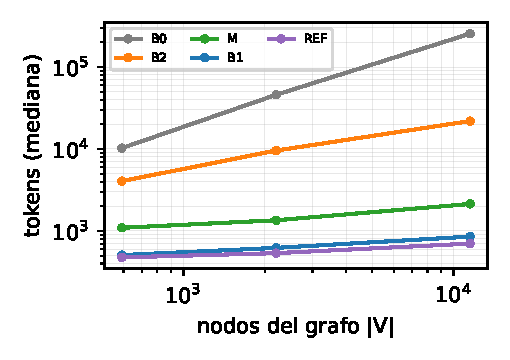
\includegraphics[width=\columnwidth]{fig/tokens_zona.pdf}
\caption{Tokens del prompt contra el tamaño del grafo (escala log--log).}\label{fig:tokens}
\end{figure}

\section{M2 --- Evaluación determinista y robusta (diseñada; parte algorítmica implementada)}
\textbf{Protocolo.} (1)~\emph{Consultas fijas}: generadas con semilla 2038 por zona, 3 zonas $\times$ 5 valores de $k\times$ 10 = 150 consultas, guardadas en el repositorio. (2)~\emph{Respuestas de referencia verificables}: $R^*$ por Held--Karp sobre distancias exactas de Dijkstra en $G$. (3)~\emph{Métricas objetivas}: validez, $\rho$, cobertura de POI (algoritmo); coincidencia de secuencia de calles y alucinaciones (LLM). (4)~\emph{Repeticiones}: 5 ejecuciones del algoritmo por consulta para tiempo (mediana) y hash SHA-256 del texto; 10 llamadas al LLM por consulta. (5)~\emph{Control}: versión de modelo fijada, plantilla fija, $T\in\{0,0.7\}$, \texttt{top\_p}$=1$, semilla, mismo tokenizador; grafos OSM cacheados en el repositorio para que los datos no cambien. (6)~Baseline sin optimizar B0.

\textbf{Determinismo contra variabilidad.} La herramienta es determinista por diseño (empates rotos por id de nodo, iteración en orden ordenado, sin aleatoriedad). Lo verificamos: en las 603 salidas del experimento (150 consultas $\times$ 4 métodos, más B0 por zona), las 5 ejecuciones dieron el mismo hash SHA-256, y dos procesos con \texttt{PYTHONHASHSEED} distinto (1 y 999) produjeron los 603 hashes, tokens y $\rho$ idénticos, igual que el barrido de $\lambda$. Por tanto, toda variación observada en la respuesta final se atribuye al LLM, que se medirá condicionando a una salida idéntica de la herramienta.

\textbf{Experimento: barrido de $\lambda$ (Fig.~\ref{fig:pareto}).} Resultado negativo. Al subir $\lambda$ de 0 a 32, la mediana de aristas del árbol baja de 100 a 81, pero los tokens \emph{suben} de 1{,}918 a 2{,}139 y $\bar\rho$ empeora de 1.028 a 1.05--1.08: no hay frente de Pareto. Diagnóstico: $\tau(e)$ cobra cada arista por igual, pero tras la contracción una avenida larga cuesta una sola línea; penalizar el número de aristas lleva al árbol a calles con menos intersecciones pero más cambios de nombre, que es lo que realmente cuesta tokens. La corrección está en Q5 (L1).
\begin{figure}[t]
\centering
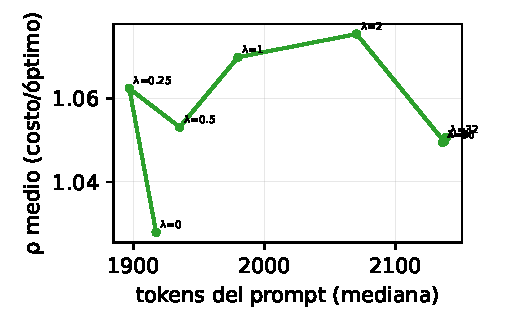
\includegraphics[width=\columnwidth]{fig/pareto.pdf}
\caption{Barrido de $\lambda$ en el corredor (20 consultas, $k=4$): tokens (mediana) contra $\bar\rho$. Más $\lambda$ no reduce tokens.}\label{fig:pareto}
\end{figure}

\section{M3 --- Preservación de calidad y asignación de recursos (planeado)}
Objetivo: $\min f_1$ sujeto a umbrales de calidad. \textbf{Umbrales:} rutas válidas 100\%; cobertura de POI 100\%; $\rho\le1.10$ en el percentil 95; restricciones $C$ respetadas 100\%; fidelidad del LLM (secuencia de calles exacta) $\ge95\%$ a $T=0$; consistencia $\ge0.9$ de acuerdo entre pares a $T=0$. \textbf{Asignación:} $B$ adaptativo según $k$ y longitud de la ruta; selección de $\lambda$ por relajación Lagrangiana; mejora L2 ($T\cup R^*$) para cumplir $\rho_{95}\le1.1$; proxy $\tau$ por cambios de calle (L1) para que $\lambda$ sí controle $f_1$. Filtro de restricciones $C$ como poda previa de aristas (peajes, tipo de vía de OSM).

\section{M4 --- Benchmark y sistema final (planeado)}
\textbf{Arquitectura final:} servidor MCP con la herramienta \texttt{plan\_route(origen, destino, pois, restricciones, presupuesto)}, un LLM con llamada a herramientas y el módulo de evaluación. \textbf{Clásicos comparados:} Dijkstra contra A$^*$ con heurística euclidiana; KMB~\cite{kmb1981} contra Mehlhorn y Dreyfus--Wagner exacto~\cite{dreyfus1971} ($\ell\le8$, para medir la brecha real de aproximación); Held--Karp contra vecino más cercano + 2-opt. \textbf{Dimensiones:} eficiencia (tokens, tiempo, memoria, costo en USD por consulta), calidad (validez, $\rho$, completitud), consistencia (acuerdo entre repeticiones), determinismo (hash de la salida, variabilidad del LLM) y escalabilidad ($n$ hasta Monterrey--Saltillo, $k$ hasta 12, lotes de consultas).

\section{Estado del repositorio y ruta de trabajo}
\textbf{Repositorio} (\texttt{steiner-llm}): \texttt{src/} (grafo, algoritmos, serializador, métodos), \texttt{tests/} (6 pruebas), \texttt{experiments/} (experimento preliminar y figuras), \texttt{data/} (grafos cacheados), \texttt{results/} (CSV) y \texttt{paper/}. \textbf{Hecho:} M1 completo sin LLM; parte algorítmica de M2. \textbf{Pendiente:} integración MCP + LLM y medición de variabilidad (semanas 1--2), M3: umbrales, restricciones, mejoras L1 y L2 (semanas 3--4), M4: clásicos, escala Monterrey--Saltillo y benchmark final (semanas 5--6).

\bibliographystyle{IEEEtran}
\bibliography{refs}

\appendix
\section{Reproducción}
Python 3.13; versiones fijadas en \texttt{requirements.txt}; grafos OSM versionados en \texttt{data/}.
\begin{verbatim}
python -m venv .venv
pip install -r requirements.txt
python -m pytest
python experiments/run_prelim.py
python experiments/plots.py
\end{verbatim}
Para el determinismo entre procesos se corre dos veces con \texttt{PYTHONHASHSEED=1} y \texttt{=999} y se comparan los hashes de la columna \texttt{sha} de \texttt{results/prelim.csv}.

\end{document}
